
\section{Theorie}
\label{sec:Theorie}

\subsection{Das Vakuum}

Ein Vakuum bezeichnet den Zustand eines Gases, wenn der Gasdruck geringer ist als der niedrigste natürlich auf der Erdoberfläche vorkommenden Atmosphärendruck\cite{Pfeiffer}. Je geringer der Druck ist, desto weniger wechselwirken die Gasteilchen untereinander, was durch die mittlere freie Weglänge beschrieben werden kann. Diese gibt an welche Strecke ein Teilchen in einem Medium zurücklegen kann, ohne mit diesem zu stoßen.\\
Ein vollkommenes Vakuum zu erzeugen ist nicht möglich, doch es gibt Pumpen die Vakuen verschiedener Qualität erzeugen können. Die Grenze zum obersten als Vakuum bezeichneten Druckbereich, dem Grobvakuum ($300 \text{ bis } \SI{1}{\milli\bar}$), ist, wie bereits erwähnt, durch den niedrigsten natürlich auf der Erde vorkommenden Druck gegeben. Ein weiterer Bereiche ist das Feinvakuum ($1 \text{ bis } \SI{e-3}{\milli\bar}$).In diesem Druckbereich liegt eine viskose laminare Strömung des abgepumpten Gases vor, das heißt auf Grund der großen Teilchenzahlen stoßen die Gasmoleküle fast nur untereinander. Im Hochvakuum ($10^{-3} \text{ bis } \SI{e-7}{\milli\bar}$) und Ultrahochvakuum ($10^{-7} \text{ bis } \SI{e-12}{\milli\bar}$) liegt eine molekulare Strömung vor. Die Teilchen wechselwirken kaum noch untereinader, sodass die mittlere freie Weglänge groß wird \cite{Pfeiffer}.\\
Benötigt wurde ein Vakuum beispielsweise in frühen Glühlampen. In der modernen Physik findet es vor allem Anwendung in Teilchenbeschleunigern, damit die dort beschleunigten Teilchenpakete nicht durch Kollisionen mit Gasteilchen verloren gehen.\\
Das Ergebnis der Vakuumerzeugung hängt auch vom Rezipienten ab. Abgesehen von fehlender Abdichtung der Ventile und Pumpen, gibt es virtuelle Lecks, die nicht von undichten Stellen herrühren, sondern bau- und lagerungsbedingt bei einem Rezipienten auftreten. Sie entstehen dadurch, dass Gase, die sich an den Innenwänden des Rezipienten angelagert haben, wieder entweichen (Desorption) oder dass bei der Herstellung mit Gasen gefüllte Hohlräume entstanden sind, die durch die Wände in den zu evakuierenden Raum diffundieren.

\subsection{Arten der Vakuumerzeugung}

Grundsätzlich lassen sich Vakuumpumpen in zwei Kategorien einteilen.
Bei Speicherpumpen wird das im Rezipienten befindliche Gas in einem mit der Pumpe verbundenen Behältnis oder Medium zwischengespeichert, weshalb auf Grund der begrenzten Kapazität nur kleinere Gasmengen abgepumpt werden können.
Bei Transportpumpen hingegen wird das Gas über die Pumpe in die Außenluft abgeleitet. Sie lassen sich deshalb für beliebig große Gasmengen verwenden \cite{Jena}.\\
Transportpumpen lassen sich in zwei Pumpentypen aufteilen: Bei einer Verdrängerpumpe wird das Gas zunächst in einen abgeschlossenen Kolben gesaugt und anschließend an die Außenluft abgegeben. Kinetische Vakuumpumpen beschleunigen das Gas mittels mechanischer Arbeit oder eines gerichteten Dampfstrahls in Pumprichtung \cite{Pfeiffer}.\\
Die in diesem Versuch betrachteten Drehschieber- und Turbomolekularpumpe sind Transportpumpen.

\subsubsection{Die Drehschieberpumpe}

Eine Drehschieberpumpe besteht wie in Abbildung \ref{fig:DSP} zu sehen aus einer zylindrischen Pumpkammer (1), einem zylindrischen Rotor (2), durch Federn an die Wand gedrückte Drehschieber, die die Kammer in zwei Halbräume teilt, und einem Ablassventil (4). Aus dem Rezipienten (R) strömt das Gas in die Kammer, wird komprimiert und durch den Überdruck am Ventil an die Außenluft abgegeben \cite{Jena}.\\
So kann ein Rezipientengasdruck $p\approx \SI{0,5e-1}{\milli\bar}$ (Feinvakuum) erzeugt werden.
In diesem Druckbereich liegt eine viskose laminare Strömung des abgepumpten Gases vor, sodass der Innendurchmesser der Rohre gering gewählt werden kann.
\begin{figure}
\centering
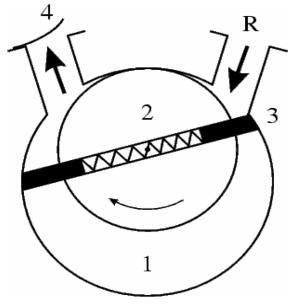
\includegraphics[scale=0.5]{content/images/Drehschieber.jpg}
\caption{Schematischer Aufbau einer Drehschieberpumpe \cite{Jena}.}
\label{fig:DSP}
\end{figure}

\subsubsection{Die Turbomolekularpumpe(Turbopumpe)}

Bei einer Turbopumpe ähnelt der Rotor einer mehrstufigen Turbine mit schaufelähnlichen Scheiben, während zwischen den Rotorscheiben spiegelverkehrte Stator-Schaufeln fest angebracht sind.\\
Der Rotor ist meist auf der Vorvakuum-Seite der Kammer auf einem Kugellager und auf der Hochvakuum-Seite auf einem verschleißfreien Permanentmagnetlager gelagert, um Verunreinigungen des Vakuums durch Schmierstoffe zu vermeiden \cite{Pfeiffer}. Die hohe Drehzahl führt dazu, dass sich die Schaufeln mit einer Geschwindigkeit bewegen, die in derselben Größenordnung liegt, wie die mittlere thermische Geschwindigkeit der Teilchen. Diese werden dadurch entlang der Drehrichtung beschleunigt und durch Abprallen von den Stator-Schaufeln durch die Pumpe geleitet \cite{Pfeiffer}.\\
Deshalb können mit einer Turbopumpe Enddrücke bis $p=\SI{e-11}{\milli\bar}$ (Ultrahochvakuum) erreicht werden, allerdings benötigt sie bereits ein Feinvakuum um zu arbeiten \cite{Pfeiffer}. Außerdem sind leichte Gase schwerer zu pumpen, da sie bereits im Mittel hohe Geschwindigkeiten haben und somit nur geringfügig vom Rotor beschleunigt werden können.\\
Auf Grund der geringen Teilchenzahl liegt eine molekulare Strömung vor. Die wenigen verbliebenen Teilchen prallen fast ausschließlich zwischen den Rohrwänden hin und her.

\subsection{Das Saugvermögen}
Die Pumpen werden durch ihr Saugvermögen 
\[
S=\frac{\mathrm{d}V}{\mathrm{d}t}
\]
charakterisiert.
Es beschreibt den durch die Ansaugöffnung der Pumpe fließenden Volumenstrom und kann über verschiedene Methoden bestimmt werden.

\subsubsection{Messung der p(t)-Kurve}

Nach dem Boyle'schen Gesetz für ideale Gase gilt bei einer konstanten Temperatur $T$:
\begin{equation}
p\cdot V =\text{const}\label{eq:Boyle}
\end{equation}
Eine Ableitung nach der Zeit ergibt
\[
\frac{\mathrm{d}V}{\mathrm{d}t} = S = - \frac{V}{p} \frac{\mathrm{d}p}{\mathrm{d}t}\text{.}
\]
Nach $p$ aufgelöst mit dem Rezipientenvolumen $V_.0$ und dem Anfangsdruck $p_.0$
\begin{equation}
p(t)=p_.0\exp{\left(-\frac{S}{V_.0}t\right)}\label{eq:pt1}\text{.}
\end{equation}
Unter Berücksichtigung, dass nie ein vollständiges Vakuum erreicht wird, sondern ein Enddruck $p_.E$ verbleibt:
\begin{equation}
p(t)=(p_.0-p_.E)\exp{\left(-\frac{S}{V_.0}t\right)}+p_.E\text{.}\label{eq:pt2}
\end{equation}
und damit für $S$
\begin{equation}
\ln\left(\frac{p-p_.E}{p_0-p_.E}\right) = -\frac{S}{V_0}t\text{.}\label{eq:S2}
\end{equation}

\subsubsection{Leckratenmessung}

Wenn genau soviel Gas in den Rezipienten strömt wie die Pumpe absaugen kann, stellt sich ein Gleichgewichtsdruck $p_.g$ ein. Dies ist entweder der Fall, wenn $p_.E$ erreicht ist, wobei das einströmende Gas in diesem Fall aus den virtuellen Lecks stammt, oder kann manuell über ein künstliches Leck eingestellt werden. \\
Wird die Pumpe in diesem Zustand abgeschaltet, füllt sich der Rezipient langsam wieder mit Gas und es gilt 
\[
S=\frac{Q}{p_.g}\text{.}
\]
Die Leckrate $Q$ bestimmt sich mit der Druckänderung $\Delta p$ in der Zeit $\Delta t$ nach
\[
Q=V_.0\frac{\Delta p}{\Delta t}
\]
und damit
\begin{equation}
S=\frac{V_.0}{p_.g}\cdot\frac{\Delta p}{\Delta t}\text{.}\label{eq:S}
\end{equation}
\newline\newline
Im Allgemeinen muss das bestimmte Saugvermögen einer Pumpe nicht mit den Herstellerangaben überein stimmen.
Das hängt mit dem Strömungswiderstand der Verbindungsrohre zusammen.
Experimentell kann nur das effektive Saugvermögen
\begin{equation}
S_.{eff}=\frac{S_.0\cdot L}{S_.0+L}
\end{equation}
bestimmt werden, wobei $S_.0$ das theoretische Saugvermögen und $L$ den Leitwert der Rohre angibt.
Dieser wird je nach Strömungsart anders berechnet und geht bei molekularer Strömung mit der 3. und bei laminarer viskoser Strömung mit der 4. Potenz des Rohrdurchmessers\cite{V70}.
Tendenziell muss bei molekularer Strömung somit der Rohrdurchmesser größer gewählt werden, um einen großen Leitwert zu gewährleisten.
Bei laminarer Strömung wird der Leitwert außerdem für geringe Drücke noch durch eine Proportionalität zum Druck begrenzt.

\subsection{Arten der Vakuummessung}

\subsubsection{Pirani-Vakuummeter}

Das Pirani-Vakuummeter arbeitet im Feinvakuum, also für $p\approx 10^{-1}\text{ bis }\SI{e-3}{\milli\bar}$ und nutzt, dass die Wärmeleitfähigkeit von Gasen in diesem Bereich proportional zum Druck ist. Die Wärmeleitung geschieht dabei im Wesentlichen über Stöße der Gasteilchen untereinander.\\
Es wird ein Draht in einer mit dem Rezipienten verbundenen Messröhre mit konstantem Strom erhitzt. Je niedriger der Druck, desto weniger Wärme kann abtransportiert werden, weshalb sich der Draht weiter aufheizt. Dadurch erhöht sich sein Widerstand. Über eine Wheatstone-Brücke kann dieser gemessen und so der Rezipientendruck bestimmt werden \cite{Jena}.

\subsubsection{Penning-Vakuummeter}

Das Penning- oder Kalt-Ionisations-Vakuummeter arbeitet im Hoch- und Ultrahochvakuum ($10^{-3} \text{ bis } \SI{e-12}{\milli\bar}$). Ein Glaskolben wird an den Rezipienten angeschlossen und durch natürliche Raumionisation freigewordene Elektronen werden zwischen zwei Elektroden beschleunigt. Sie können dabei weitere Elektronen ausschlagen, sodass der fließende Strom ein Maß für den Gasdruck ist. Durch einen am Kolben befestigten Permanentmagneten werden die Elektronen in eine Spiralbahn ausgelenkt und so der Weg zwischen den Elektroden - und damit die Wahrscheinlichkeit der Stoßionisation - vergrößert, um den Messbereich zu erweitern \cite{Jena}.

\subsubsection{Bayard-Alpert-Vakuummeter}

Beim Bayard-Alpert-Vakuummeter,siehe Abbildung \ref{fig:bav}, ist die Elektronenquelle eine Glühkathode (K). Die Elektronen werden zu der Anode (A) hin beschleunigt und ionisieren auf dem Weg die verbliebenen Gasteilchen. Die Ionen werden zu einer weiteren negativ geladenen Elektrode (C) beschleunigt und beim Auftreffen neutralisiert, was zu einem messbaren Strom führt. Dieses Vakummeter arbeitet im Hoch- und Ultrahochvakuum \cite{Spektrum}.
\begin{figure}
\centering
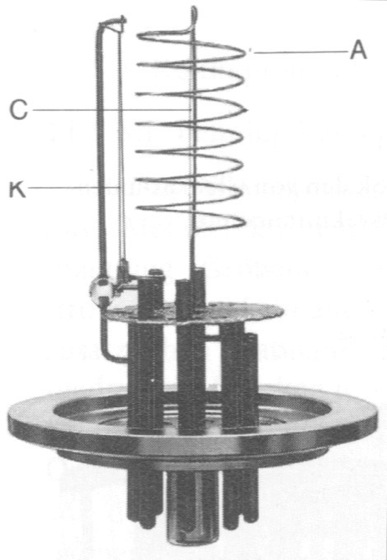
\includegraphics[scale=0.3]{content/images/bav.jpg}
\caption{Das Bayard-Alpert-Vakuummeter \cite{Spektrum}.}
\label{fig:bav}
\end{figure}